%% ============================================================ 2 PROBABILITY
\clearpage
\inchap{Probability}
\section{Basic Rules}
\begin{center}\bba\small
\begin{tabular}{|L{4.4cm}|M{5.5cm}|L{5.3cm}|}\hline
\textbf{Result} & \textbf{Formula} & \textbf{Note}\\\Xhline{2pt}
Equally likely outcomes & $\Pp{A}=\dfrac{n(A)}{n(S)}$ & $0\leqslant\Pp{A}\leqslant1$\\\hline
Complement & $\Pp{A'}=1-\Pp{A}$ & ``at least one'' $=1-\text{none}$\\\hline
Addition rule & $\Pp{A\cup B}=\Pp{A}+\Pp{B}-\Pp{A\cap B}$ & $A\cup B$: $A$ or $B$ (or both)\\\hline
Mutually exclusive & $\Pp{A\cap B}=0$ & so $\Pp{A\cup B}=\Pp{A}+\Pp{B}$\\\hline
Exhaustive & $\Pp{A\cup B}=1$ & \\\hline
\end{tabular}\end{center}
\begin{center}\ba\small
\begin{tabular}{|M{2.5cm}|M{2.5cm}|M{2.5cm}|M{2.5cm}|M{2.5cm}|}\hline
\vnn{white}{white}{white}{\sh}&\vnn{white}{\sh}{white}{white}&\vnn{white}{white}{\sh}{white}&\vnn{\sh}{white}{white}{white}&\vnn{white}{\sh}{\sh}{white}\\
$A\cap B$&$A\cap B'$&$A'\cap B$&$A'\cap B'=(A\cup B)'$&exactly one\\\hline
$\Pp{A\cap B}$&$\Pp{A}-\Pp{A\cap B}$&$\Pp{B}-\Pp{A\cap B}$&$1-\Pp{A\cup B}$&$\Pp{A}+\Pp{B}-2\Pp{A\cap B}$\\\hline
\end{tabular}\end{center}
\sidenote{The four regions add up to $1$. $(A\cup B)'=A'\cap B'$ \ and \ $(A\cap B)'=A'\cup B'$. None of these probability results is in MF27.}\par
\section{Conditional Probability}
\begin{center}\bba\small
\begin{tabular}{|M{4.4cm}|M{5.2cm}|L{5.6cm}|}\hline
\textbf{Result} & \textbf{Formula} & \textbf{Note}\\\Xhline{2pt}
Conditional probability & $\Pp{A\g B}=\dfrac{\Pp{A\cap B}}{\Pp{B}}$ & probability of $A$ given $B$ has happened; $\Pp{B}\neq0$\\\hline
Multiplication rule & $\Pp{A\cap B}=\Pp{A\g B}\Pp{B}=\Pp{B\g A}\Pp{A}$ & used along a tree branch\\\hline
Complement given $B$ & $\Pp{A'\g B}=1-\Pp{A\g B}$ & \\\hline
Warning & $\Pp{A\g B}\neq\Pp{B\g A}$ & different denominators\\\hline
\end{tabular}\end{center}
\begin{center}\begin{tikzpicture}[scale=1]
\node[anchor=east,font=\small] at (-0.4,0){reduced sample space:};
\draw (0,-1.0) rectangle (3.8,1.0);\draw (1.6,0) circle (0.85);\draw[fill=blue!10] (2.4,0) circle (0.85);
\node[font=\small] at (0.5,0.7){$A$};\node[font=\small] at (3.4,0.7){$B$};
\begin{scope}\clip (1.6,0) circle (0.85);\fill[blue!30] (2.4,0) circle (0.85);\end{scope}
\draw (1.6,0) circle (0.85);\draw (2.4,0) circle (0.85);
\node[right,font=\small] at (4.1,0){$\Pp{A\g B}=\dfrac{\text{shaded}}{\text{whole circle }B}$};
\end{tikzpicture}\end{center}
\section{Independent and Mutually Exclusive Events}
\begin{center}\ba\small
\begin{tabular}{|M{2.4cm}|M{6.6cm}|M{6.2cm}|}\hline
 & \textbf{Independent} & \textbf{Mutually exclusive}\\\Xhline{2pt}
Meaning & one event does not change the probability of the other & cannot both happen\\\hline
Test & \textbullet\ $\Pp{A\cap B}=\Pp{A}\Pp{B}$\newline\textbullet\ $\Pp{A\g B}=\Pp{A}$\newline\textbullet\ $\Pp{B\g A}=\Pp{B}$ & \textbullet\ $\Pp{A\cap B}=0$\newline\textbullet\ $\Pp{A\cup B}=\Pp{A}+\Pp{B}$\\\hline
Venn & circles overlap, $\Pp{A\cap B}=\Pp{A}\Pp{B}$ & circles do not overlap\\\hline
\end{tabular}\end{center}
\begin{info}[title=Note]
\begin{itemize}\setlength{\itemsep}{0pt}\item If $A$, $B$ are independent, so are $A$ and $B'$, $A'$ and $B$, $A'$ and $B'$.\item If $\Pp{A}>0$ and $\Pp{B}>0$, events cannot be both independent and mutually exclusive: $\Pp{A\cap B}=0\neq\Pp{A}\Pp{B}$.\item To show independence, show $\Pp{A\cap B}=\Pp{A}\Pp{B}$; \emph{do not} assume it from the wording.\item Independence cannot be detected from the shape of the Venn diagram: it generally looks the same as a Venn diagram in which $A$ and $B$ are not independent.\end{itemize}
\end{info}
\noindent\exlab Given that $A$ is independent of $B$, prove that $A'$ is independent of $B'$.
\cdisp{\Pp{A'\cap B'}&=1-\Pp{A\cup B}\\&=1-\Pp{A}-\Pp{B}+\Pp{A\cap B}\\\because\ \Pp{A\cap B}&=\Pp{A}\Pp{B}\\\therefore\ \Pp{A'\cap B'}&=1-\Pp{A}-\Pp{B}+\Pp{A}\Pp{B}\\&=\bigl(1-\Pp{A}\bigr)\bigl(1-\Pp{B}\bigr)\\&=\Pp{A'}\Pp{B'}\\\therefore\ &A',\,B'\text{ are independent}}
\Needspace{18\baselineskip}
\section{Tree Diagrams}
Multiply along branches ($\cap$); add across leaves ($\cup$). Branches from one node sum to $1$. Without replacement: probabilities in the second stage \textbf{change}.\par\smallskip
\begin{center}\begin{tikzpicture}[x=1cm,y=0.85cm,
 every node/.style={font=\small},
 lf/.style={right,font=\small},ed/.style={midway,font=\small,fill=white,inner sep=1pt}]
\node[circle,fill,inner sep=1.3pt] (o) at (0,0){};
\node (r) at (3,1.9){$R$};\node (b) at (3,-1.9){$B$};
\draw (o)--(r) node[midway,above left,inner sep=1.5pt]{$\dfrac58$};\draw (o)--(b) node[midway,below left,inner sep=1.5pt]{$\dfrac38$};
\node (rr) at (6.5,3.0){$R$};\node (rb) at (6.5,1.0){$B$};\node (br) at (6.5,-1.0){$R$};\node (bb) at (6.5,-3.0){$B$};
\draw (r)--(rr) node[midway,above left,inner sep=1.5pt]{$\dfrac47$};\draw (r)--(rb) node[midway,below left,inner sep=1.5pt]{$\dfrac37$};
\draw (b)--(br) node[midway,above left,inner sep=1.5pt]{$\dfrac57$};\draw (b)--(bb) node[midway,below left,inner sep=1.5pt]{$\dfrac27$};
\node[lf] at (rr.east){$\ \dfrac58\times\dfrac47=\dfrac{5}{14}$};
\node[lf] at (rb.east){$\ \dfrac58\times\dfrac37=\dfrac{15}{56}$};
\node[lf] at (br.east){$\ \dfrac38\times\dfrac57=\dfrac{15}{56}$};
\node[lf] at (bb.east){$\ \dfrac38\times\dfrac27=\dfrac{3}{28}$};
\node[above,font=\footnotesize] at (1.5,3.7){$1^{\text{st}}$};\node[above,font=\footnotesize] at (4.8,3.7){$2^{\text{nd}}$};
\end{tikzpicture}\end{center}
\sidenote{Bag: 5 red, 3 blue; 2 drawn without replacement.}\par
\cdisp{\Pp{\text{different colours}}&=\dfrac{5}{8}\times\dfrac{3}{7}+\dfrac{3}{8}\times\dfrac{5}{7}\\&=\dfrac{15}{56}+\dfrac{15}{56}\\&=\dfrac{15}{28}\\\Pp{\text{1st }R\g\text{2nd }B}&=\dfrac{\Pp{\text{1st }R\text{ and 2nd }B}}{\Pp{\text{2nd }B}}\\&=\dfrac{\Pp{R,B}}{\Pp{R,B\text{ or }B,B}}\\&=\dfrac{\dfrac{15}{56}}{\dfrac{15}{56}+\dfrac{6}{56}}\\&=\dfrac{5}{7}}
\section{Tables of Outcomes and Counting Methods}
\noindent\begin{minipage}[c]{0.43\textwidth}
\centering\renewcommand{\arraystretch}{1.05}\small
\begin{tabular}{c|cccccc}
$+$&1&2&3&4&5&6\\\hline
1&2&3&4&5&6&\cellcolor{blue!25}7\\
2&3&4&5&6&\cellcolor{blue!25}7&8\\
3&4&5&6&\cellcolor{blue!25}7&8&9\\
4&5&6&\cellcolor{blue!25}7&8&9&10\\
5&6&\cellcolor{blue!25}7&8&9&10&11\\
6&\cellcolor{blue!25}7&8&9&10&11&12
\end{tabular}\par\smallskip
{\footnotesize two dice: $n(S)=36$}
\end{minipage}\hfill
\begin{minipage}[c]{0.54\textwidth}
\cdisp{\Pp{\text{sum}=7}&=\dfrac{6}{36}=\dfrac16\\\Pp{\text{sum}\geqslant10}&=\dfrac{6}{36}=\dfrac16\\\Pp{\text{sum}=7\g\text{a }3\text{ shown}}&=\dfrac{2}{11}}
\end{minipage}\par\smallskip
\noindent\exlab There are $6$ men and $10$ women. $5$ people are chosen. Find the probability that the group has $3$ men.

\noindent\begin{minipage}[t]{0.6\textwidth}
(a)
\cdisp{\Pp{3M,2W}&=\dfrac{6}{16}\times\dfrac{5}{15}\times\dfrac{4}{14}\times\dfrac{10}{13}\times\dfrac{9}{12}\times{\color{blue}\dfrac{5!}{2!\,3!}}\\&=\dfrac{15}{728}\times{\color{blue}10}\\&=\dfrac{75}{364}}
\end{minipage}\hfill\vrule\hfill
\begin{minipage}[t]{0.36\textwidth}
(b)
\cdisp{\Pp{3\text{ men}}&=\dfrac{\nCr{6}{3}\times\nCr{10}{2}}{\nCr{16}{5}}\\&=\dfrac{20\times45}{4368}\\&=\dfrac{75}{364}}
\end{minipage}
\section{Further Question Types}
\begin{center}\renewcommand{\arraystretch}{1.08}\footnotesize
\begin{tabular}{|L{4.6cm}|L{10.6cm}|}\hline
\textbf{Type} & \textbf{Method}\\\Xhline{2pt}
Range of $\Pp{A\cap B}$ & Label $\Pp{A\cap B}=x$, then label all other areas in terms of $x$. Let each area $\geqslant0$ and solve.\\\hline
Games: ``first to win'', taking turns & list the winning sequences; the game can go on forever; the probabilities form a \textbf{GP}; $S_{\infty}=\dfrac{a}{1-r}$ ($|r|<1$)\\\hline
Venn diagram with unknowns ($x$, $y$) & label the regions (2 or 3 events) with $x$, $y$, \ldots; regions add to $1$; use some other info in the equation to link $x$ and $y$; every region $\geqslant0$ gives the greatest / least value\\\hline
\end{tabular}\end{center}
\noindent\begin{minipage}[t]{0.48\textwidth}
\exlab $\Pp{A}=0.45$, $\Pp{B}=0.7$. Find the range of values of $\Pp{A\cap B}$.
\cdisp{\text{let }\Pp{A\cap B}&=x\\\Pp{A\cap B'}&=0.45-x\\\Pp{A'\cap B}&=0.7-x\\\Pp{A'\cap B'}&=1-(0.45-x)-(0.7-x)-x\\&=x-0.15\\\because\ \text{each area}&\geqslant0\\\therefore\ 0.15&\leqslant\Pp{A\cap B}\leqslant0.45}
\end{minipage}\hfill
\begin{minipage}[t]{0.48\textwidth}
\exlab $A$, $B$ take turns to roll a die, $A$ first; first six wins
\cdisp{\Pp{A\text{ wins}}&=\frac16+\left(\frac56\right)^{2}\frac16+\left(\frac56\right)^{4}\frac16+\cdots\\&=\dfrac{1/6}{1-25/36}\\&=\dfrac{6}{11}}
\end{minipage}
